\documentclass[12pt]{article}

\usepackage{fancyhdr}
\usepackage{amssymb}
\usepackage{amsthm}
\usepackage{amsfonts}
\usepackage{mathtools}
\usepackage{array}
\usepackage{systeme}
\usepackage{geometry}
\usepackage{enumitem}
\usepackage{ dsfont }
\usepackage{listings}
\usepackage{tikz}
\usetikzlibrary{arrows,decorations.pathmorphing,backgrounds,positioning,fit}
\usetikzlibrary{automata, positioning}
\usetikzlibrary{calc}
\usepackage[utf8]{inputenc}
  \geometry{
    left = 2.5cm,
    right = 2.5cm,
    includeheadfoot, top = 1.5cm, bottom = 1.5cm,
    headsep = 1.3cm,
    footskip = 1.2cm
  }

% Inline fraction %
\newcommand*\rfrac[2]{{}^{#1}\!/_{#2}}
\newcommand{\lincom}[4]{\mathit{{#1}{\underline{#2}}}+\mathit{{#3}{\underline{#4}}}}
\newcommand*{\QEDA}{\hfill\ensuremath{\blacksquare}}
\newcommand*{\QEDB}{\hfill\ensuremath{\square}}
\newcommand{\MU}[1]{\mathit{\underline{#1}}}

\newcommand{\DS}{\displaystyle}
\newcommand{\bb}[1]{\mathbb{#1}}

% Absolute value: \abs{x} => |x|
\newcommand{\abs}[1]{\left|#1\right|}

% Function: \func{f}{X}{Y} => f : X -> Y
\newcommand{\func}[3]{#1 : #2 \rightarrow #3}
% Function to R: \func{f}{X} => f : X -> R
\newcommand{\functoR}[2]{#1 : #2 \rightarrow \mathbb{R}}
% Function to N: \func{f}{X} => f : X -> N
\newcommand{\functoN}[2]{#1 : #2 \rightarrow \mathbb{N}}
% Function from R to R: \func{f} => f : R -> R
\newcommand{\funcR}[1]{#1 : \mathbb{R} \rightarrow \mathbb{R}}

% Limits and convergence
\newcommand{\limn}{\lim_{n \to \infty}}
\newcommand{\limh}{\lim_{h \to 0}}
\newcommand{\limsupn}{\limsup_{n \to \infty}}
\newcommand{\liminfn}{\liminf_{n \to \infty}}
\newcommand{\limx}[1]{\lim_{x \to #1}}
\newcommand{\tounif}{\xrightarrow{unif.}}

% Sums and series
\newcommand{\sumn}[1]{\sum_{k=1}^n #1}
\newcommand{\series}[1]{\sum_{k=1}^\infty #1}
\newcommand{\seriec}[1]{\sum_{k=m}^n #1}
\newcommand{\pseries}[1]{\sum_{n=0}^\infty #1}

% Intervals
% Closed-closed interval [a,b]
\newcommand{\intcc}[1]{\left[#1\right]}
% Open-closed interval (a,b]
\newcommand{\intoc}[1]{\left(#1\right]}
% Closed-open interval [a,b)
\newcommand{\intco}[1]{\left[#1\right)}
% Open-open interval (a,b)
\newcommand{\intoo}[1]{\left(#1\right)}

% Sets
\newcommand{\N}{\mathbb{N}}
\newcommand{\Z}{\mathbb{Z}}
\newcommand{\Q}{\mathbb{Q}}
\newcommand{\R}{\mathbb{R}}
\newcommand{\e}{\varepsilon}

\lhead{Alexander Fischer, Camillo Malnati, Federico Pfahler, Aldo Gabriele di Rosa}
\chead{}
\rhead{}
\rfoot{\thepage}
\cfoot{}
\lfoot{\today}
\pagestyle{fancy}

\begin{document}
  \begin{center}
    \LARGE{\textbf{Citybike Pollution Data Collection}}
  \end{center}
  \section{Introduction}
  \newpage
  \section{Architecture}
  \begin{figure}[ht]
    \centering
    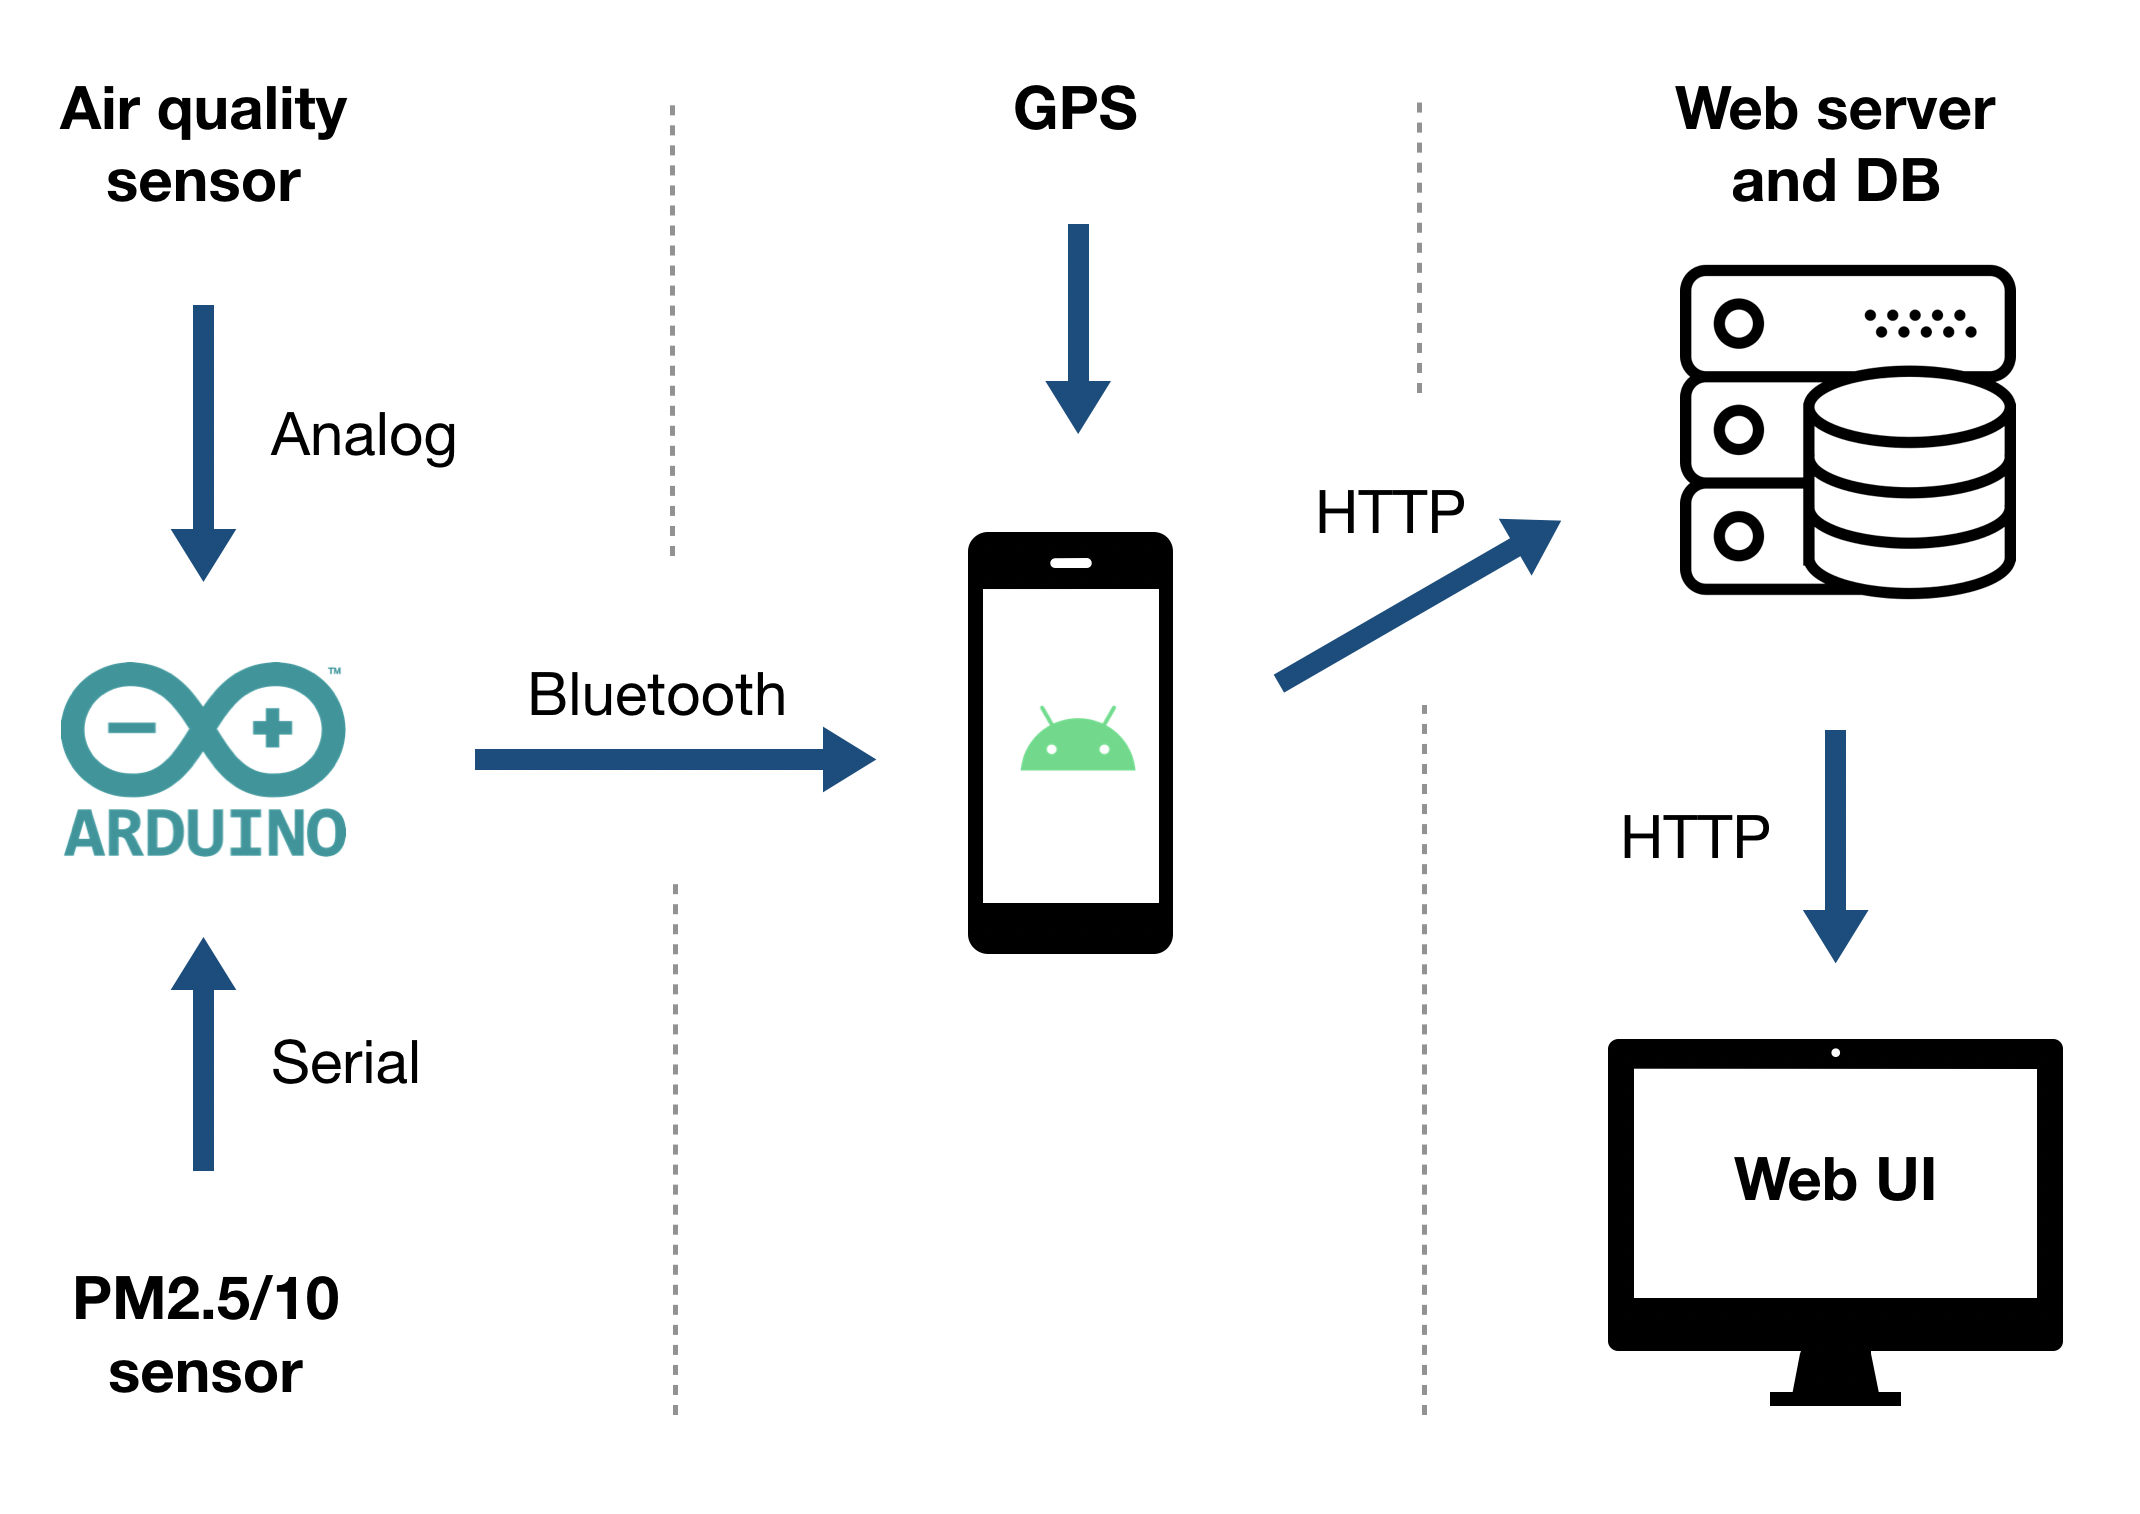
\includegraphics[width=\textwidth]{images/architecture.png}
    \caption{An overview of the main components in our system.}
    \label{fig:architecture}
  \end{figure}
  \subsection{Sensors}
  \subsubsection{Air quality}
  \subsubsection{Pollution (PM2.5/PM10)}
  \subsection{Android application}
  The goal of the Android application is to act as a gateway between the Arduino board that collects pollution data from sensors and the web application that stores and visualizes the aggregated data. While forwarding pollution measures, it also adds the current location coordinates obtained from the phone's GPS sensor.

  The application runs on a mobile phone (in our demo a Huawei P10 lite running Android 8.0) that is connected via Bluetooth to the Arduino Nano 33 BLE board, as well as with an active GSM connection.
  Its source code is based on an example application, \verb|BluetoothLeGatt|, bundled with the Android SDK, that allows to scan for Bluetooth Low Energy devices and connect to them. 

  What we added to that code was to, on every message received from the Arduino board, retrieve the location coordinates (using the Android FusedLocation API) and send that data together with the pollution information to a web server as a JSON object by performing a POST request. An example of such JSON object is shown in Figure~\ref{lst:json-packet}. On the other hand, the message sent from the board is structured as follows: \verb|123,12,5;|. It contains the measurements from the air quality sensor, as well as the two measured values from the PM2.5/10 sensor.

  %TODO: add screenshots of app

  \begin{figure}[h]
    \centering
    \begin{verbatim}
{
  "createdAt": "2019-12-13T09:22:49.824Z",
  "lat": 46.0037,
  "long": 8.9511 ,
  "bikeId" : "00002add-0000-1000-8000-00805f9b34fb",
  "pm10": 5,
  "pm25": 12,
  "airQuality": 123
}
    \end{verbatim}
  \caption{An example JSON object containing the pollution measurements and location}\label{lst:json-packet}
  \end{figure}

  \subsection{Web application}
  \newpage
  \section{Conclusions}
  

\end{document}
